\documentclass[12pt]{article}
\usepackage{graphicx}
\usepackage{url}
\usepackage{multirow}
\usepackage{listings}
\usepackage{xcolor}
\lstset { %
   language=C++,
   backgroundcolor=\color{black!5}, % set backgroundcolor
   basicstyle=\footnotesize,% basic font setting
}


\title{Why would you sort when you know where things approximately belong?}
\author{Peter Taraba \footnote{Berkeley, CA}}

\begin{document}

	
	\maketitle
	
	\begin{abstract}
  		We introduce statistical sorting, which is close to $O(n)$ time complexity on average (as it really is $O(n \log \log n)$ complexity), and compare it with mainstream C++ std (standard template library) sort, which has on average $O(n \log n)$ time complexity. We show it on three different distributions - uniform, Gauss and an additional one. Statistical sorting is usually called nested bucket sorting, but unlike standard bucket sorting which divides into a constant number of $m$ buckets, to achieve $O(n \log \log n)$ complexity, nesting and variable number of buckets of size $\sqrt{n}$ are needed.
	\end{abstract}
	
	\section{Introduction}
	
		Currently, the most popular algorithm for sorting is the quick sort algorithm, which has $O(n \log n)$ time complexity on average \cite{numrec} and in the worst case $O(n^2)$. This publication introduces statistical sorting which is closer to $O(n)$ than $O(n \log n)$ time complexity (it really is $O(n \log \log n)$ complexity). In C++, the std::sort() function is implemented using the Intro Sort Algorithm, which combines three standard sorting algorithms: insertion sort, quick sort, and heap sort \cite{cppsort}. On average, they all have $O(n \log n)$ time complexity \cite{wikisort}.
		
		In section 2, we introduce the statistical algorithm, in section 3 we show simple implementation in C++, in section 4 we compare it with C++ std sort, in section 5 we do a more robust complexity analysis of std sort and statistical sorting, in section 6 we talk about simple parallelization of the statistical algorithm and finally in section 7, we draw conclusions and discuss future work.

	\section{Stat Sort Algorithm}
	
		The simple idea behind statistical sorting is to go through the vector, find its minimum and maximum value (which is $O(n)$), and then split the vector into many tiny ones, which will be sorted either by the same algorithm (in case size of the vector is more than a chosen threshold; for this publication, we chose threshold 10) or by standard sorting algorithms (C++ std sort, etc). For this publication, we chose the number of vectors we split the initial vector of size $s$ as $\sqrt{s}$. This was satisfactory to achieve better time complexity performance (closer to $O(n)$) than other sorting algorithms, which usually have on average $O(n \log n)$ time complexity. We show this on several examples - uniform distribution, Gaussian distribution (\cite{gauss}) as well as one additional distribution. As the implementation of the statistical sorting is very short in C++, instead of describing it in too many details, we provide the entire algorithm in the following section. The algorithm is also known as nested bucket sorting, but instead of a constant number of buckets $m$, we subdivide the vectors into variable size $\sqrt{n}$ buckets, where $n$ is the length of the vectors.
		
		
	\section{Stat Sort Algorithm Implementation in C++}
	
	C++ implementation of the basic statistical sorting is as follows:
	
		\begin{lstlisting}
void statsort(vector<double> &vec, double min, double max)
{
    int memsize = sqrt(vec.size());
    std::vector<double> *myvectors = 
        new std::vector<double>[memsize];

    for(long int i=0;i<vec.size();i++)
    {
        long int where = (int)((vec[i]-min) * 
            (memsize + 0.0) / (max-min));

        myvectors[where].push_back(vec[i]);
    }

    for(long int i=0;i<memsize;i++)
    {
        if(myvectors[i].size()>10)
        {
            statsort(myvectors[i], min+(i+0.0)*(max-min)/memsize, 
                min+(i+1.0)*(max-min)/memsize);
        }
        else
        {
            std::sort (myvectors[i].begin(), myvectors[i].end());
        }
    }

    vec.clear();
    for(long int i=0;i<memsize;i++)
    {
        for(int j=0;j<myvectors[i].size();j++)
        {
            vec.push_back(myvectors[i][j]);
        }
    }
    delete[] myvectors;
}

void statsort(vector<double> &vec)
{
    double min, max;

    min = std::numeric_limits<double>::max();
    max = std::numeric_limits<double>::lowest();

    for(long int i=0;i<vec.size();i++)
    {
        if(min>vec[i])
        {
            min = vec[i];
        }
        if(max<vec[i])
        {
            max = vec[i];
        }
    }

    max += 0.0001 * (max-min);
    statsort(vec, min, max);
}
		\end{lstlisting}
	
	\section{Std Sort vs Stat Sort}
	
		Measured times of std sort and stat sort are in figure \ref{fig1}, \ref{fig2} and \ref{fig3}, as well as theoretical $O(n \log n)$, $O(n \log \log n)$ and $O(n)$ time complexity determined by linear regression and minimum residual. While for uniform and additional distribution, the expected complexity is confirmed, for Gaussian it is actually better than the expected complexity (for stat sort it is $O(n)$ instead of $O(n \log \log n)$ and for std sort it is $O(n \log \log n)$ instead of $O(n \log n)$). This can be due to many reasons such as chosen sizes of vectors, operating systems, memory allocations, etc. This is also summarized in table \ref{table2}.

		\begin{figure}
		\begin{center}
			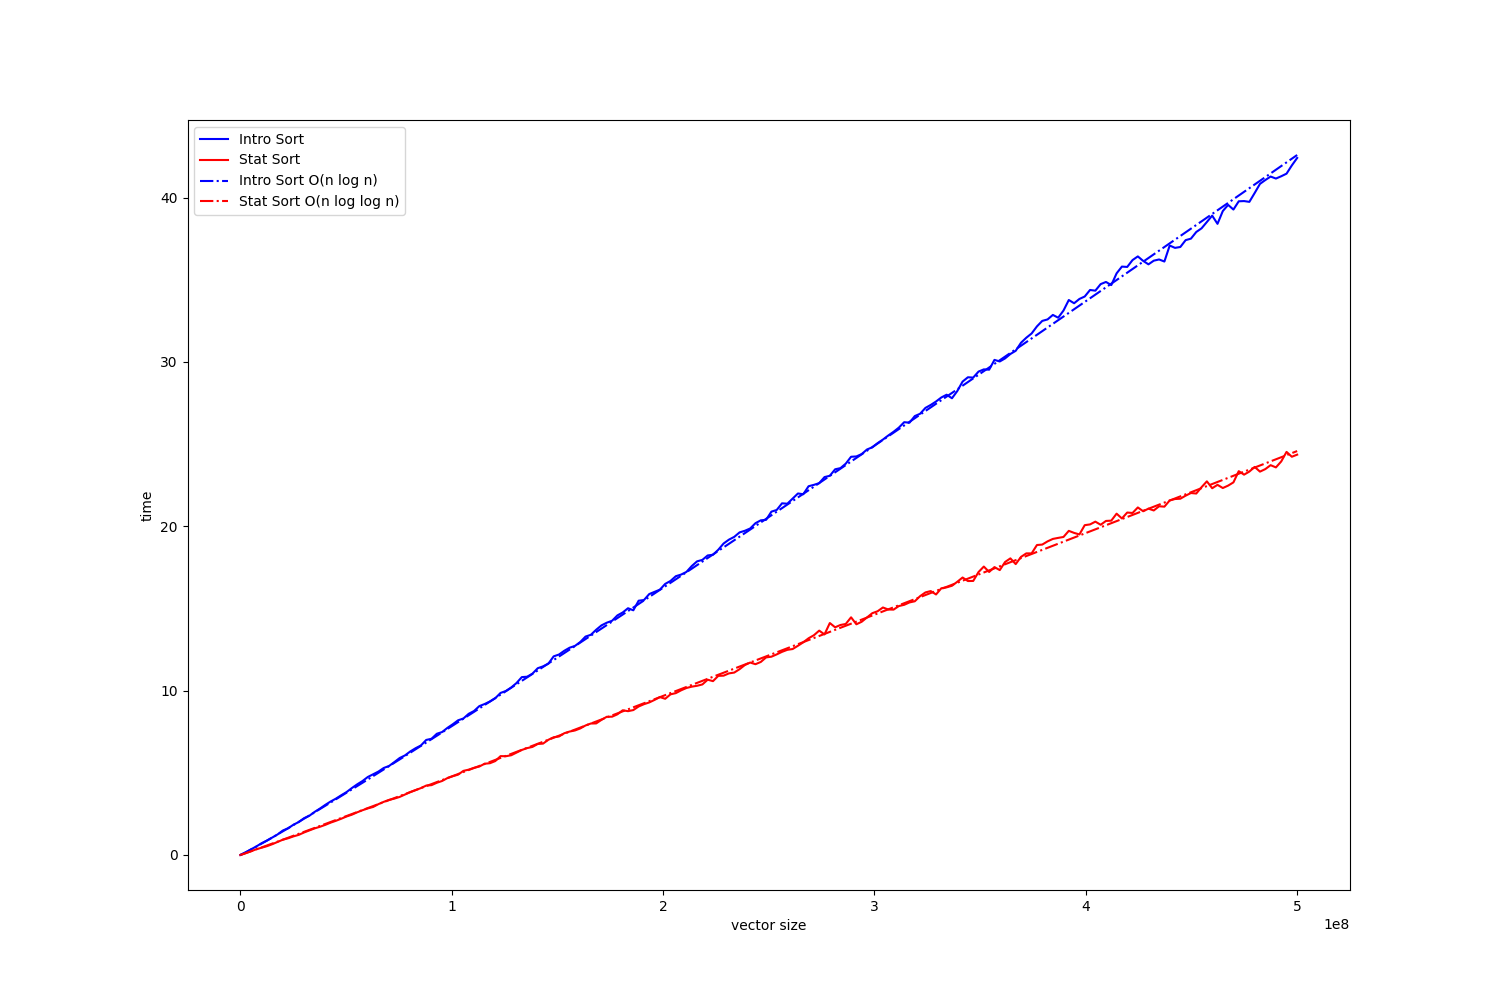
\includegraphics[width=0.8\textwidth]{fig_perf_uniform}
		\end{center}
			\caption{C++ std sort (blue) vs C++ stat sort (red) for uniform distribution vector. Full lines are measured times, the dashed blue line is $O(n \log n)$ for C++ std sort, and the dashed red line is $O(n)$ for C++ stat sort determined by residuals from linear regression fit.}
		
		\label{fig1}
		\end{figure}		

		\begin{figure}
		\begin{center}
			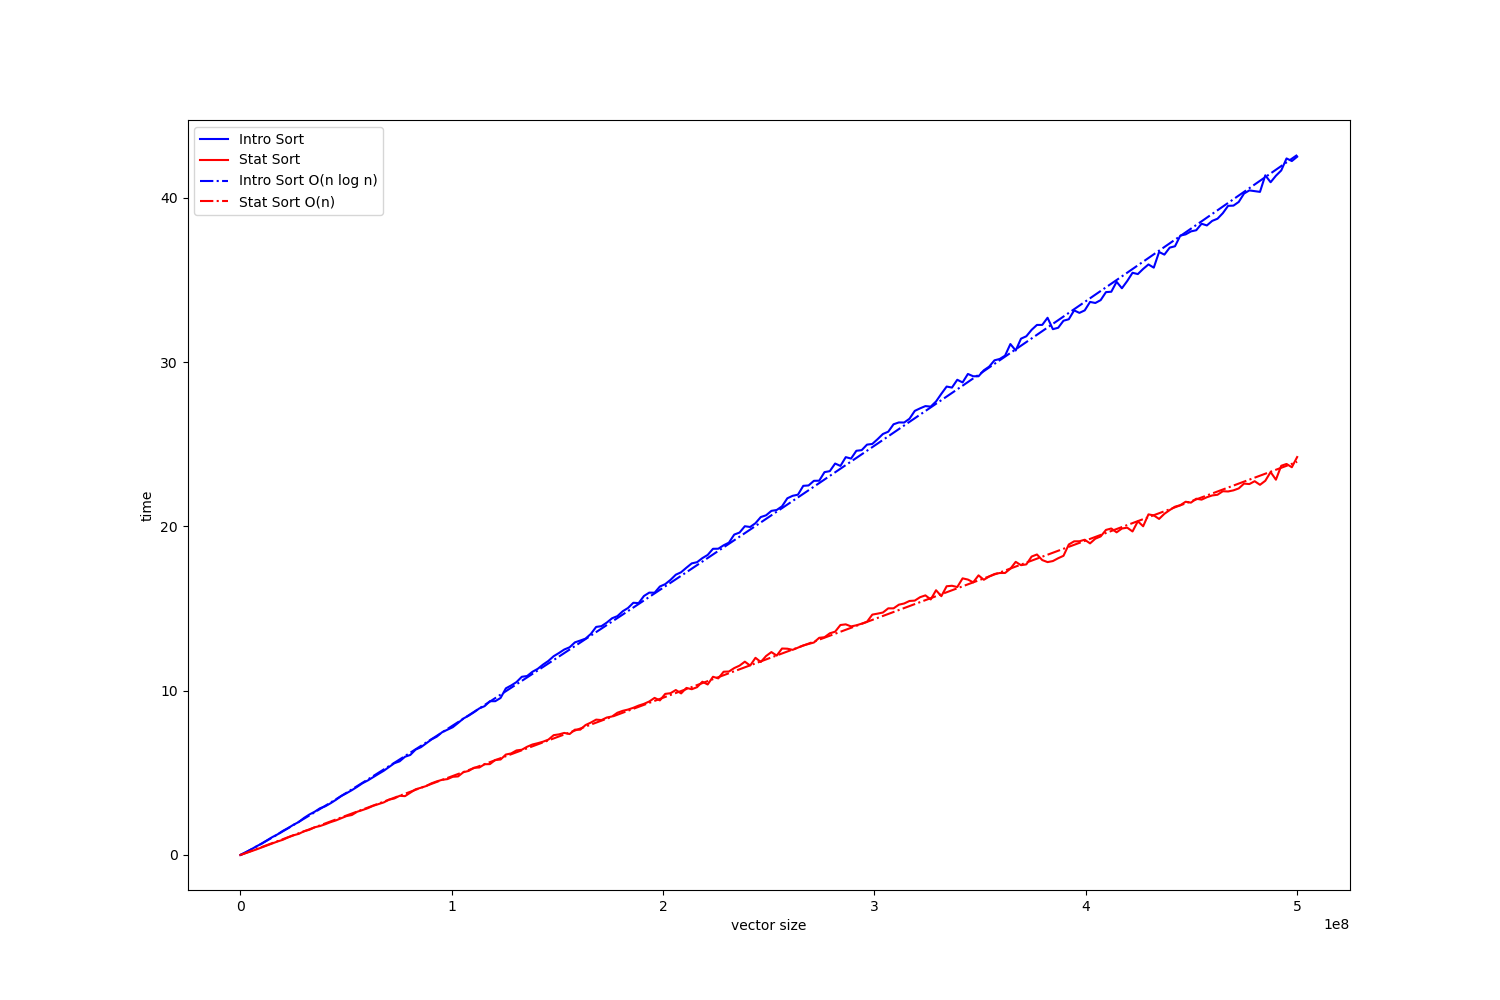
\includegraphics[width=0.8\textwidth]{fig_perf_gauss}
		\end{center}
			\caption{C++ std sort (blue) vs C++ stat sort (red) for Gaussian distribution vector. Full lines are measured times, the dashed blue line is $O(n \log n)$ for C++ std sort, and the dashed red line is $O(n)$ for C++ stat sort determined by residuals from linear regression fit.}
		
		\label{fig2}
		\end{figure}		

		\begin{figure}
		\begin{center}
			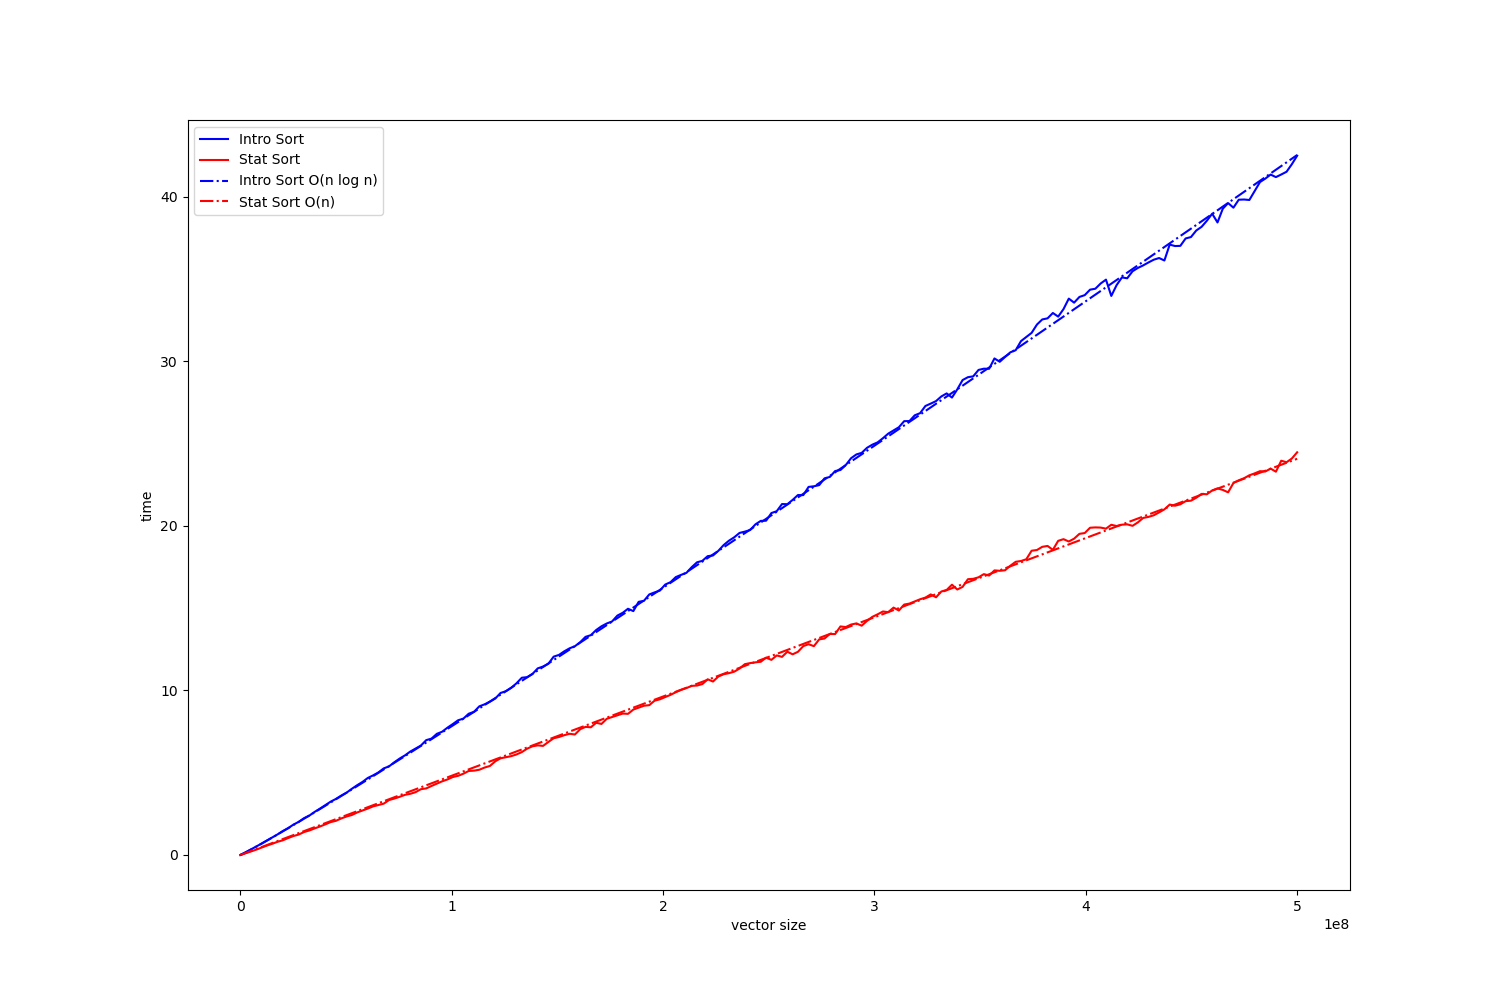
\includegraphics[width=0.8\textwidth]{fig_perf_weird}
		\end{center}
			\caption{C++ std sort (blue) vs C++ stat sort (red) for an additional distribution vector. Full lines are measured times, the dashed blue line is $O(n \log n)$ for C++ std sort, and the dashed red line is $O(n)$ for C++ stat sort determined by residuals from linear regression fit.}
		
		\label{fig3}
		\end{figure}		
		
		\begin{figure}
		\begin{center}
			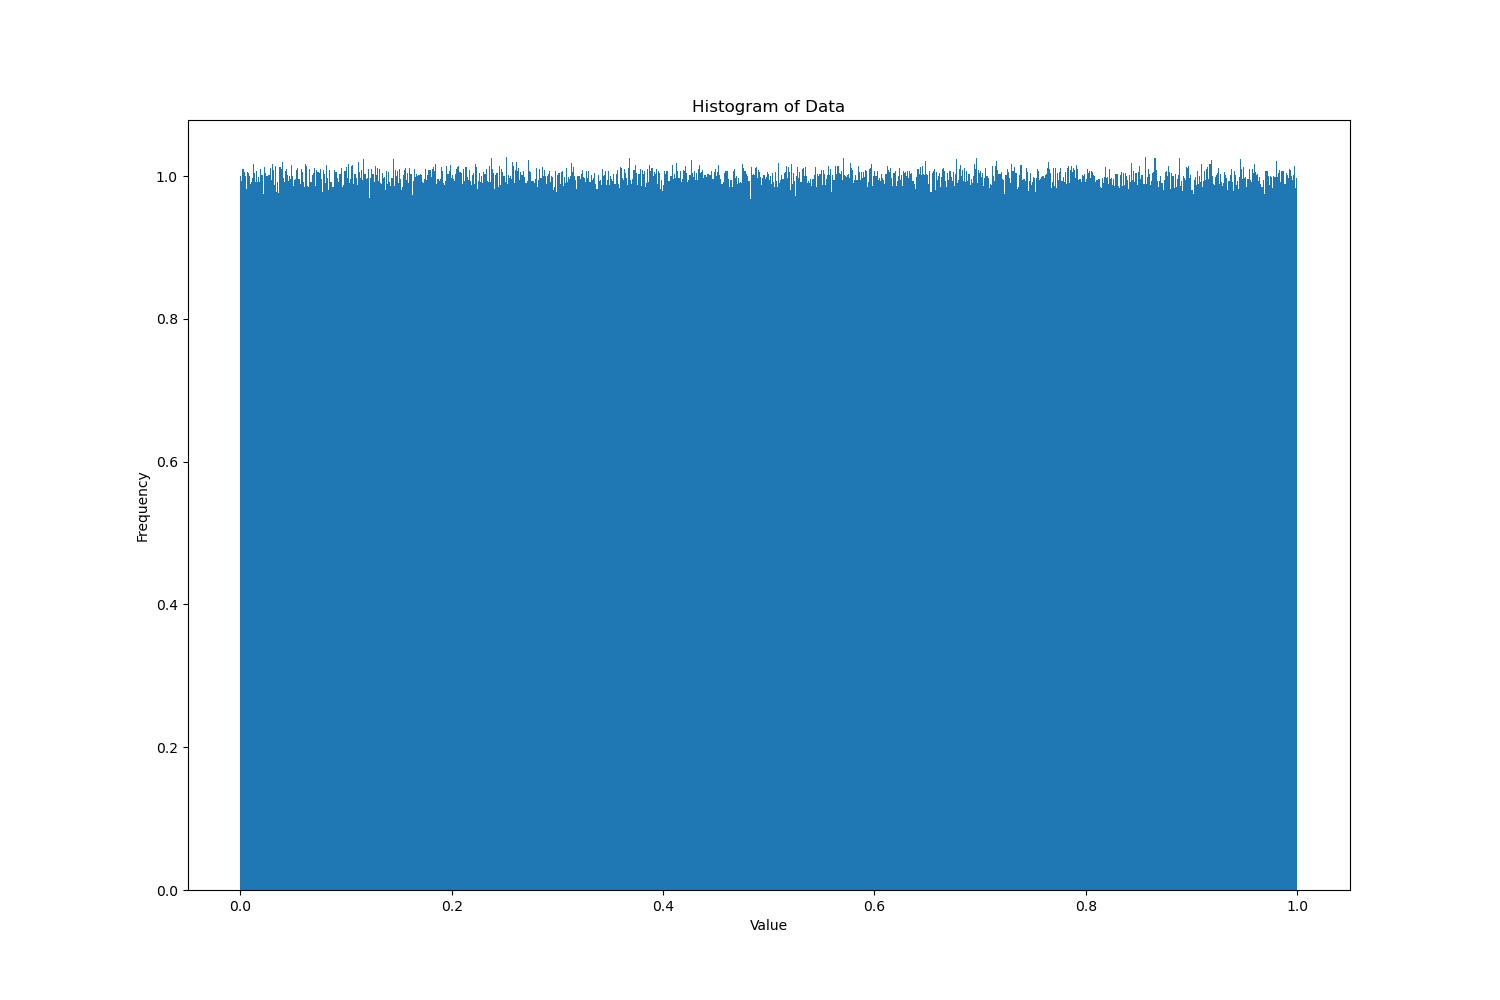
\includegraphics[width=0.32\textwidth]{fig_dist_norm}
			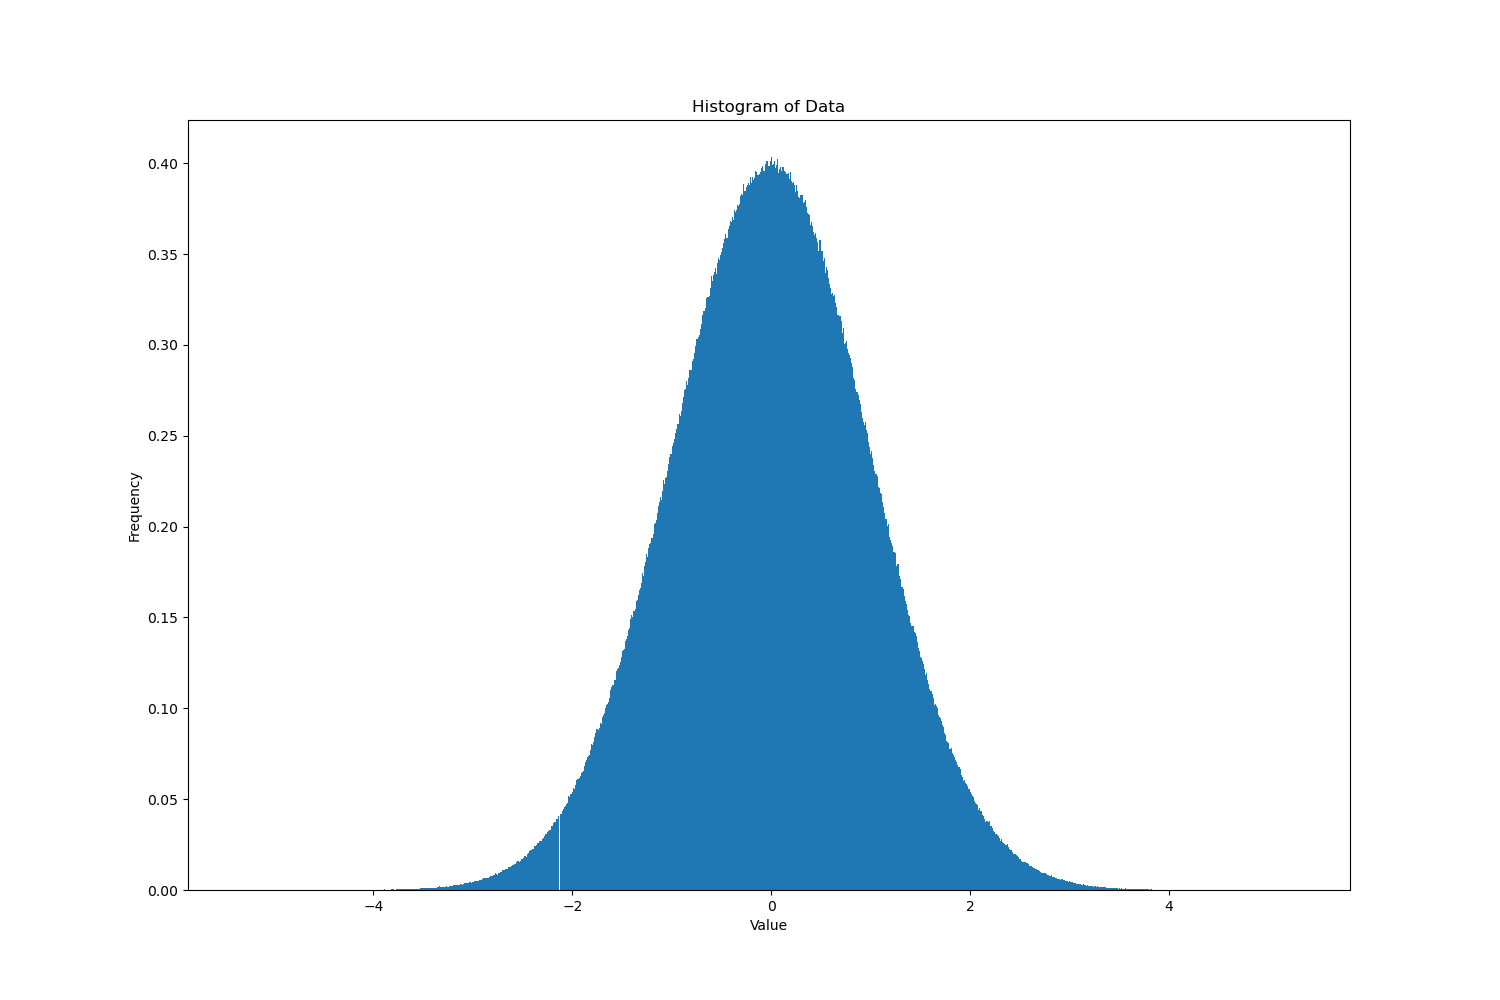
\includegraphics[width=0.32\textwidth]{fig_dist_gauss}
			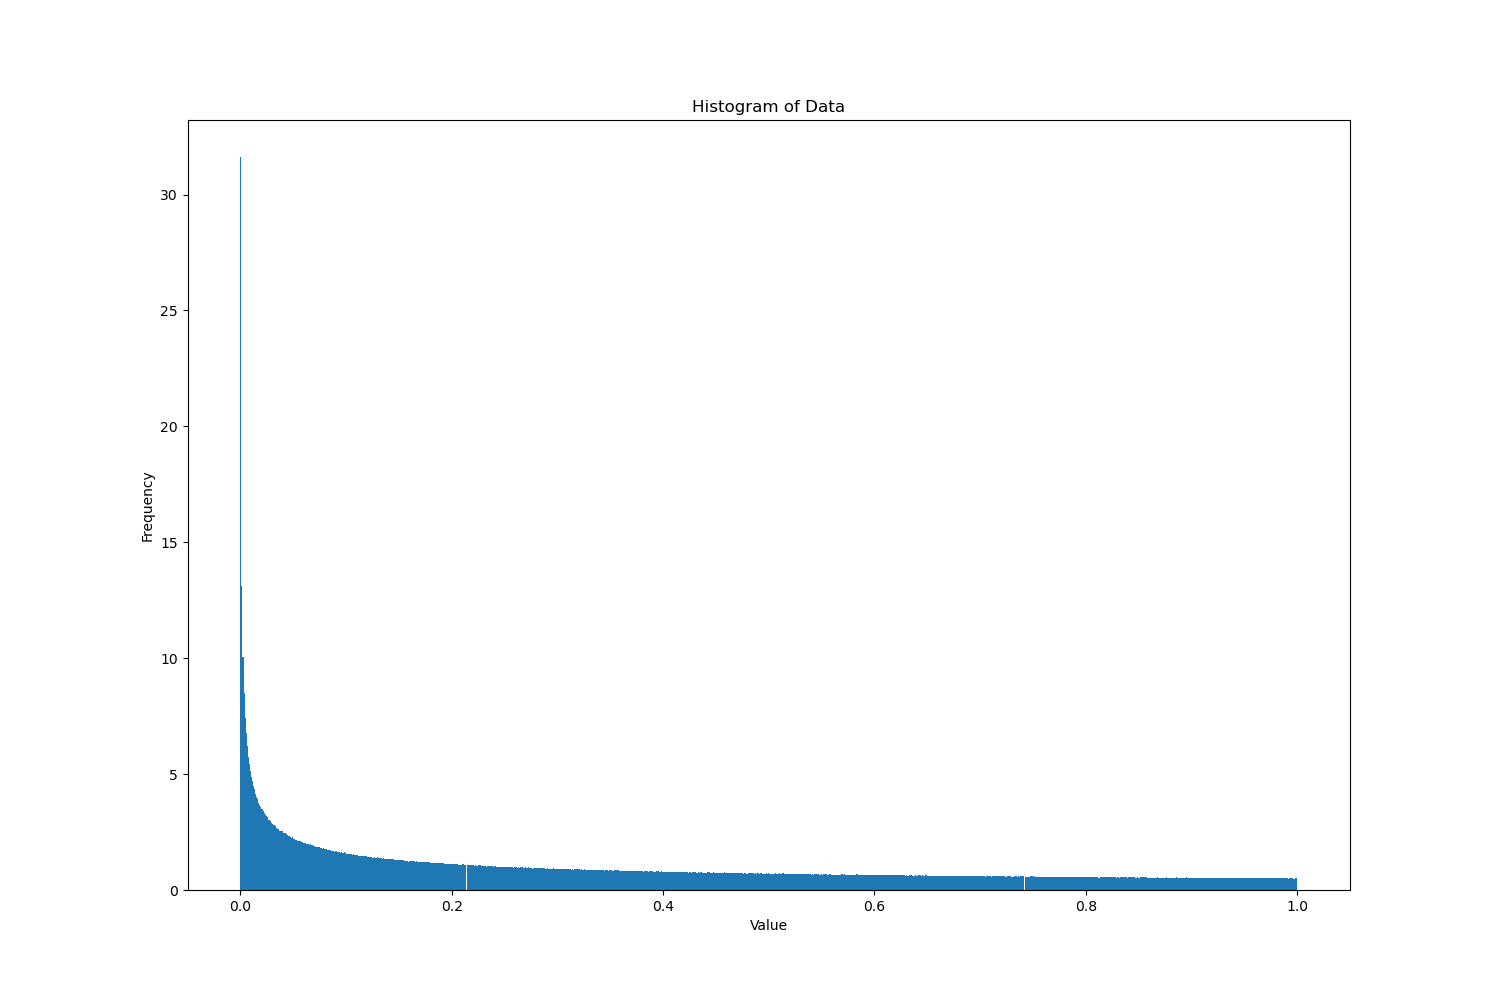
\includegraphics[width=0.32\textwidth]{fig_dist_weird}
		\end{center}
		\caption{Three distributions tested. From left - uniform, Gaussian, and an additional one.}
		\label{fig4}
		\end{figure}		
						
		The reason why statistical sorting is close to $O(n$) for $n = n_1 n_2$ is because of
		\[
		O(n_1 n_2 \log n_2) \approx O(n_1 n_2) = O(n),
		\]
		as $\log n_2$ is approximately constant for small $n_2$. In case larger $n$ would be measured (over 500000000), it could become again $O(n \log n)$ (without nesting). For our measurements, we cannot go over 500000000 due to the memory limitations of most Linux users (16 GB of RAM memory). 
		As we do recursion in the sorting algorithm, we can show close to $O(n)$ time complexity as follows:
		\[
		O(n^{1/2} (n^{1/2} \log n^{1/2})),
		\]
		and as $n^{1/2} \log n^{1/2}$ can be sorted again with recursion, we get
		\[
		O(n^{1/2} n^{1/4} (n^{1/4} \log n^{1/4})),
		\]
		and using recursion again and again will get us
		\[
		O(n^{1/2} n^{1/4} n^{1/8} ...) = O(n).
		\]
		So theoretically, using recursion we should get close to $O(n)$ even for vectors beyond 500000000.
        
        Now let's analyze time complexity for statistical sorting more precisely. If the constant $m$ would be used for the amount of buckets, we could write
        \[
        k m^l \approx n, 
        \]
        where $l$ is a number of nestings, $n$ is the size of the original vector and $k$ is a threshold, for which we do not nest anymore. From the equation, we get $l \approx \log n$ and because of the additional fact that we have to go $l$ times through a vector of size $n$, we would end up again with complexity $O(n l) = O(n \log n)$.

        Because we use non-constant size of buckets, we can write
        \[
        {k^2}^l \approx n.
        \]
        From this, we get $l \approx \log \log n$. Hence the final complexity is $O(n l) = O(n \log \log n)$, which is closer to $O(n)$ than $O(n \log n)$.
			
		Table \ref{table1} contains selected measurements for time execution and table \ref{table2} contains residuals for determining the time complexity of both compared algorithms. All three distributions can be seen in figure \ref{fig4}.
		
		\begin{table}
		\caption{Times for Quick \& Stat Sort for various vector sizes}
		\begin{center}
		\begin{tabular}{ |c|c|c| }
		
		\hline
		
		size & Quick Sort time & Stat Sort time \\

		\hline\hline		
		
		10000		& 1.15760485641658E-08	& 0 \\
		10060050    & 8.27546318760142E-06	& 5.12730912305415E-06 \\
		100510502	& 9.20717575354502E-05	& 5.54861180717126E-05 \\
		201011005	& 0.000190925929928198	& 0.000110023145680316 \\
		301511507	& 0.000290057876554783	& 0.000171666666574311 \\
		402012010	& 0.000397928241000045	& 0.000232824073464144 \\
		500000000	& 0.00049090277752839	& 0.00028194444894325 \\

		\hline
		\end{tabular}
		\end{center}
		\label{table1}
		\end{table}


		\begin{table}
		\caption{Determining time complexity of Std \& Stat Sort through residuals for all three cases - Uniform, Gaussian and additional distribution}
		\begin{center}
		\begin{tabular}{ |c|c|c|c| }
		\hline
		
		Case & Time complexity & Std Sort residual & Stat Sort residual \\

		\hline\hline
		
		\multirow{3}{*}{Uniform} & $O(n)$ &		27.80140662 &  7.98515784  \\
	     & $O(n \log n)$ & \textbf{13.80724414}		& 11.03394399 \\
          & $O(n \log \log n)$ & 15.39617211 & \textbf{6.43584778} \\

        \hline\hline

		\multirow{3}{*}{Gauss} & $O(n)$ &		25.42304015 & \textbf{6.8534117}   \\
		 & $O(n \log n)$ & 15.96232138		& 23.65668998  \\        
         & $O(n \log \log n)$ & \textbf{14.51259308} & 10.09139965 \\

        \hline\hline

		\multirow{3}{*}{Additional} & $O(n)$ & 29.83324385	 & 5.69070067    \\
		 & $O(n \log n)$ & \textbf{12.27187648} & 9.75464218  \\
         & $O(n \log \log n)$ & 16.23142872 & \textbf{4.56616269} \\        

		\hline
		\end{tabular}
		\end{center}
		\label{table2}
		\end{table}

		
		The entire code for the plots in figure \ref{fig1}, \ref{fig2}, \ref{fig3}, \ref{fig4} and tables \ref{table1} and \ref{table2} can be found on github \cite{peta78}.

    \section{Further complexity analysis of sorting algorithms}

    As the previous section showed, the complexity analysis for 200 measurements and one parameter estimation can draw suspicious results, as for the Gaussian distribution conclusion was that std sort is closer to $O(n \log \log n)$ and statistical sorting is closer to $O(n)$, which based on theoretical understanding of algorithms is not correct. Hence, there seems to be a need for more robust complexity detection. Hence, for confirmation of $O(n)$, we use formula
    \[
    \frac{T(n_1)}{T_(n_2)} \approx \frac{n_1}{n_2},
    \]
    for confirmation of $O(n \log n)$ we use
    \[
    \frac{T(n_1)}{T_(n_2)} \approx \frac{n_1 \ln n_1}{n_2 \ln n_2},
    \]
    and for confirmation of $O(n \log \log n)$ we use
    \[
    \frac{T(n_1)}{T_(n_2)} \approx \frac{n_1 \ln \ln n_1}{n_2 \ln \ln n_2}.
    \]
    If we use all combinations of all measurements, instead of relying only on 200 measurements, we get $\frac{198 \cdot 199}{2} = 19701$ measurements and a more robust estimation. (As the first measurement is 0 for statistical sorting, we cannot use it). We look at absolute values of differences between measurements (left-hand side of previous equations) and theoretical estimations (right-hand side of previous equations). We look at the number of wins (which complexity was closer for each case) as well as averages of these differences and we plot also distributions of these $19701$ measurements. This is summarized in table \ref{table3} and distribution figures \ref{fig5}, \ref{fig6} and \ref{fig7} and confirms that std sort has $O(n \log n)$ time complexity and stat sort has $O(n \log \log n)$ time complexity with only exception for Gaussian case and number of wins, but this is disproved by average and distribution graphs. These figures \ref{fig5}, \ref{fig6} and \ref{fig7} also explain why $O(n \log \log n)$ time complexity is closer to $O(n)$ than $O(n \log n)$ time complexity (in the right portion of figures look that for statistical sorting red distribution is better than green distribution).

		\begin{table}
		\caption{Determining time complexity of Std \& Stat Sort through wins (max number) and absolute error average (min value) for all three cases - Uniform, Gaussian and additional distribution}
		\begin{center}
		\begin{tabular}{ |c|c|c|c|c|c| }
		\hline
		%Std Sort residual & Stat Sort residual
        \multirow{2}{*}{Case} & \multirow{2}{*}{Time complexity} & \multicolumn{2}{|c|}{std sort} & \multicolumn{2}{|c|}{stat sort} \\
        
		 &  & Wins & Average & Wins & Average \\

		\hline\hline
		
		\multirow{3}{*}{Uniform} & $O(n)$ & 2273  & 0.8203 & 5100 & 0.4004 \\
	     & $O(n \log n)$ & \textbf{14140} & \textbf{0.1153} & 5792 & 0.5254\\
          & $O(n \log \log n)$ & 3288 & 0.5241 & \textbf{8809} & \textbf{0.1351}\\

        \hline\hline

		\multirow{3}{*}{Gauss} & $O(n)$ & 3114 & 0.8323 & \textbf{11549} & 0.2508 \\
		 & $O(n \log n)$ & \textbf{13276} & \textbf{0.1292} & 2639 & 0.6969 \\        
         & $O(n \log \log n)$ & 3311 & 0.5372 & 5513 & \textbf{0.1133} \\

        \hline\hline

		\multirow{3}{*}{Additional} & $O(n)$ & 2151 & 0.8006 & 5505 & 0.3639  \\
		 & $O(n \log n)$ & \textbf{14927} & \textbf{0.1323} & 4733 & 0.5603 \\
         & $O(n \log \log n)$ & 2623 & 0.5043 & \textbf{9463} & \textbf{0.0954} \\        

		\hline
		\end{tabular}
		\end{center}
		\label{table3}
		\end{table}

        \begin{figure}
		\begin{center}
			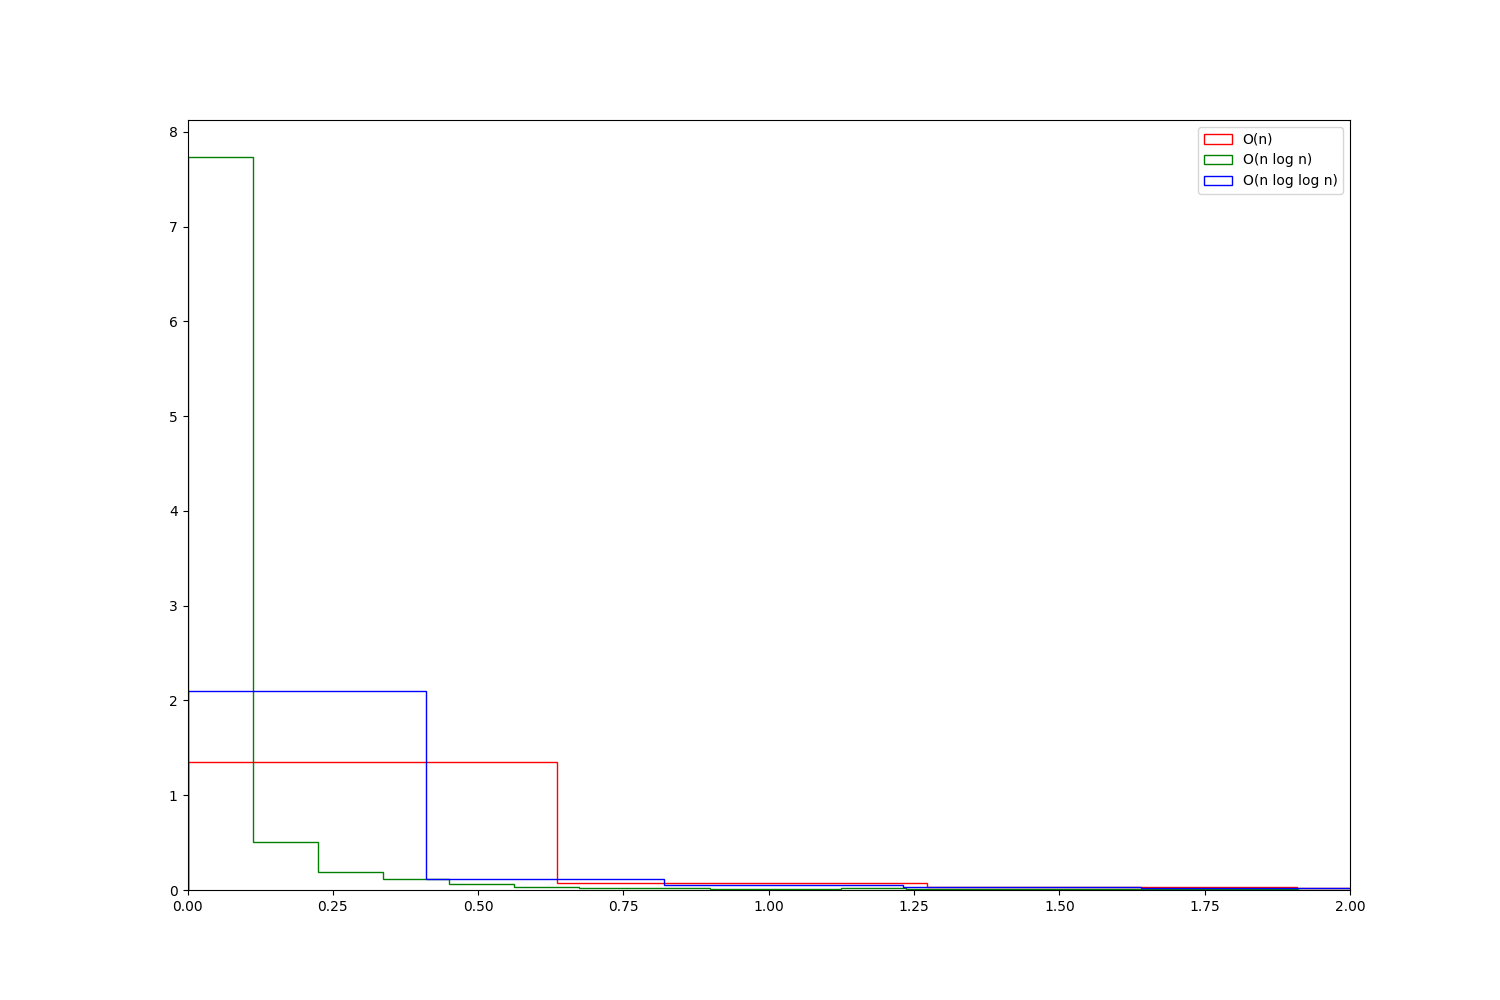
\includegraphics[width=0.44\textwidth]{fig_dist_anal_uniform_stdsort.png}
			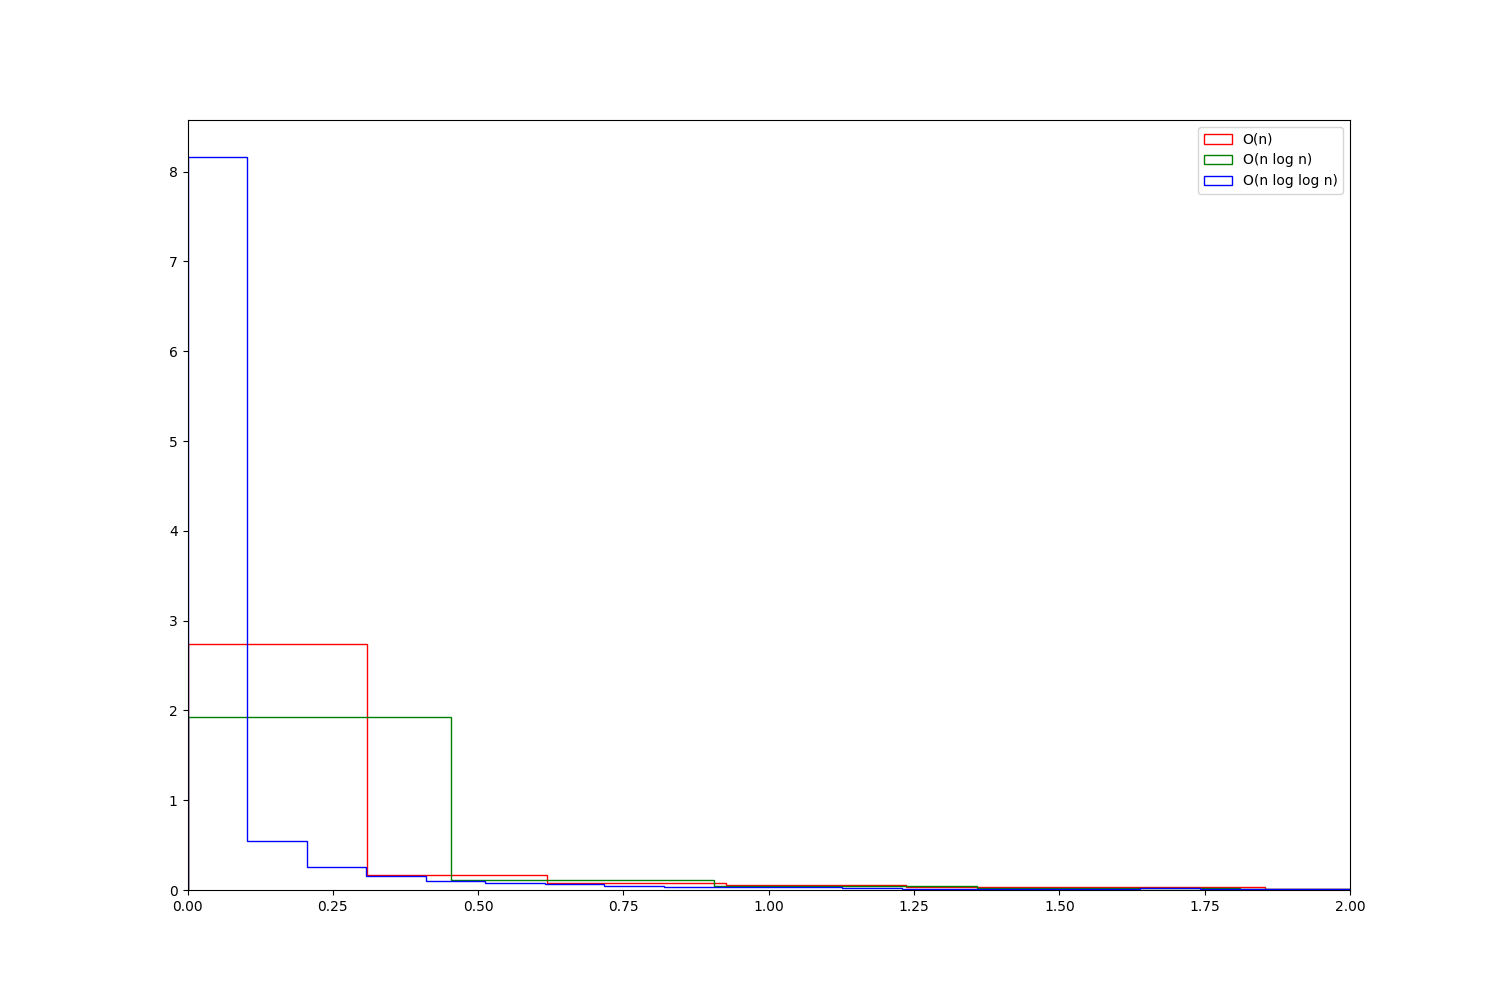
\includegraphics[width=0.44\textwidth]{fig_dist_anal_uniform_statsort.png}
		\end{center}
		\caption{Analysis of algorithm complexity for std sort (left) and stat sort (right) and confirmation that std sort is $O(n \log n)$ and stat sort is $O(n \log \log n)$ for uniform distribution.}
		\label{fig5}
		\end{figure}	

        \begin{figure}
		\begin{center}
			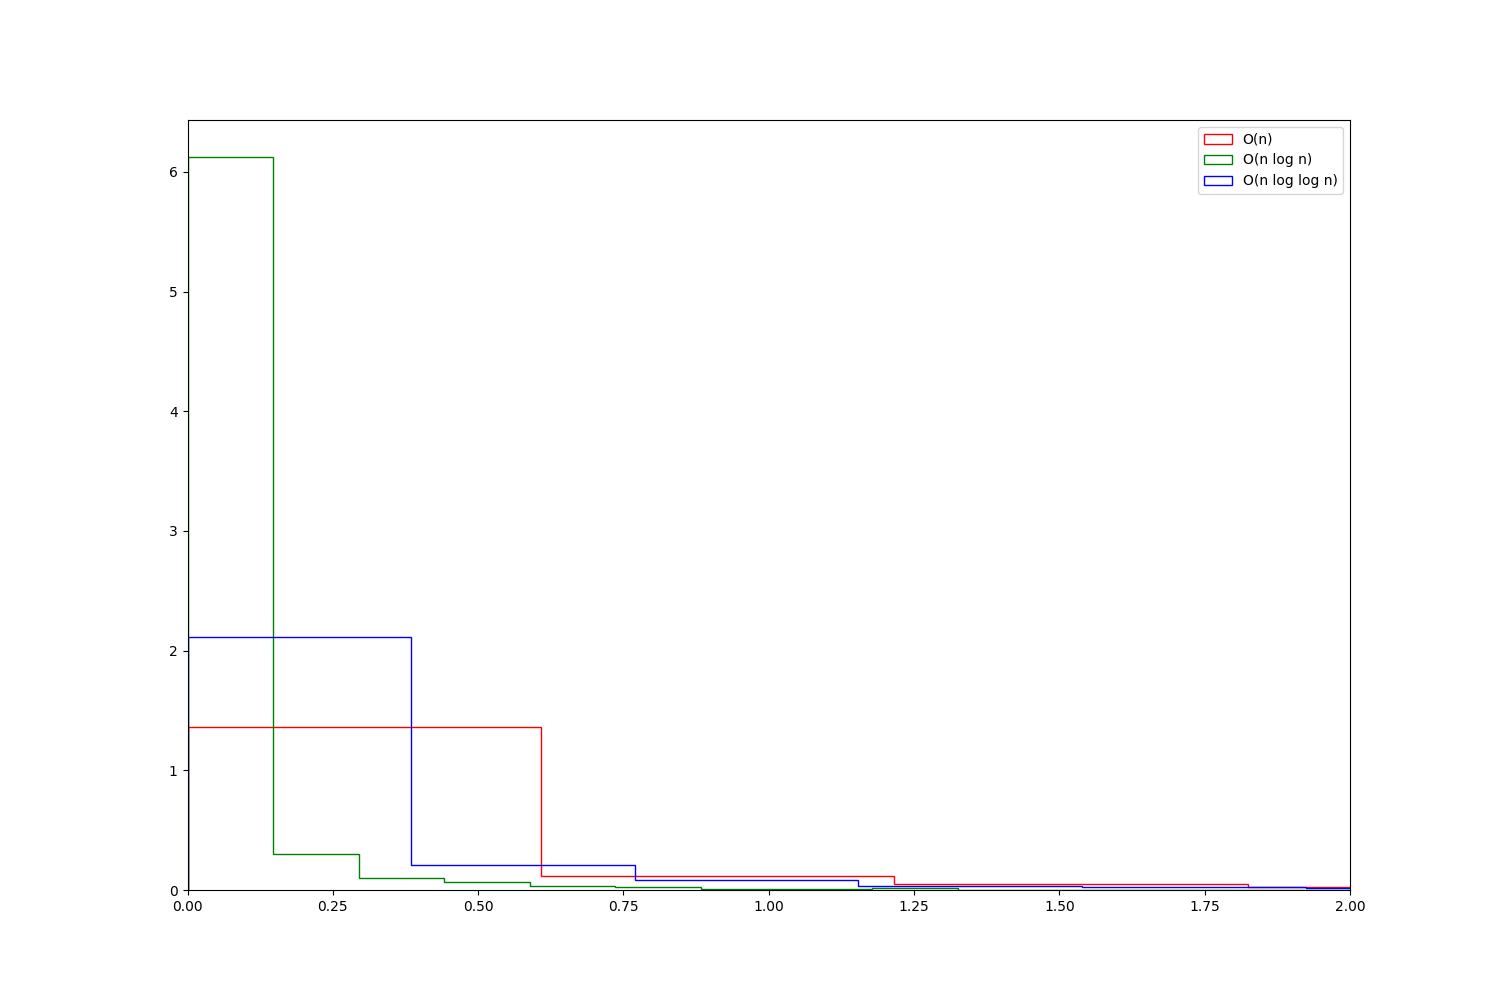
\includegraphics[width=0.44\textwidth]{fig_dist_anal_gauss_stdsort.png}
			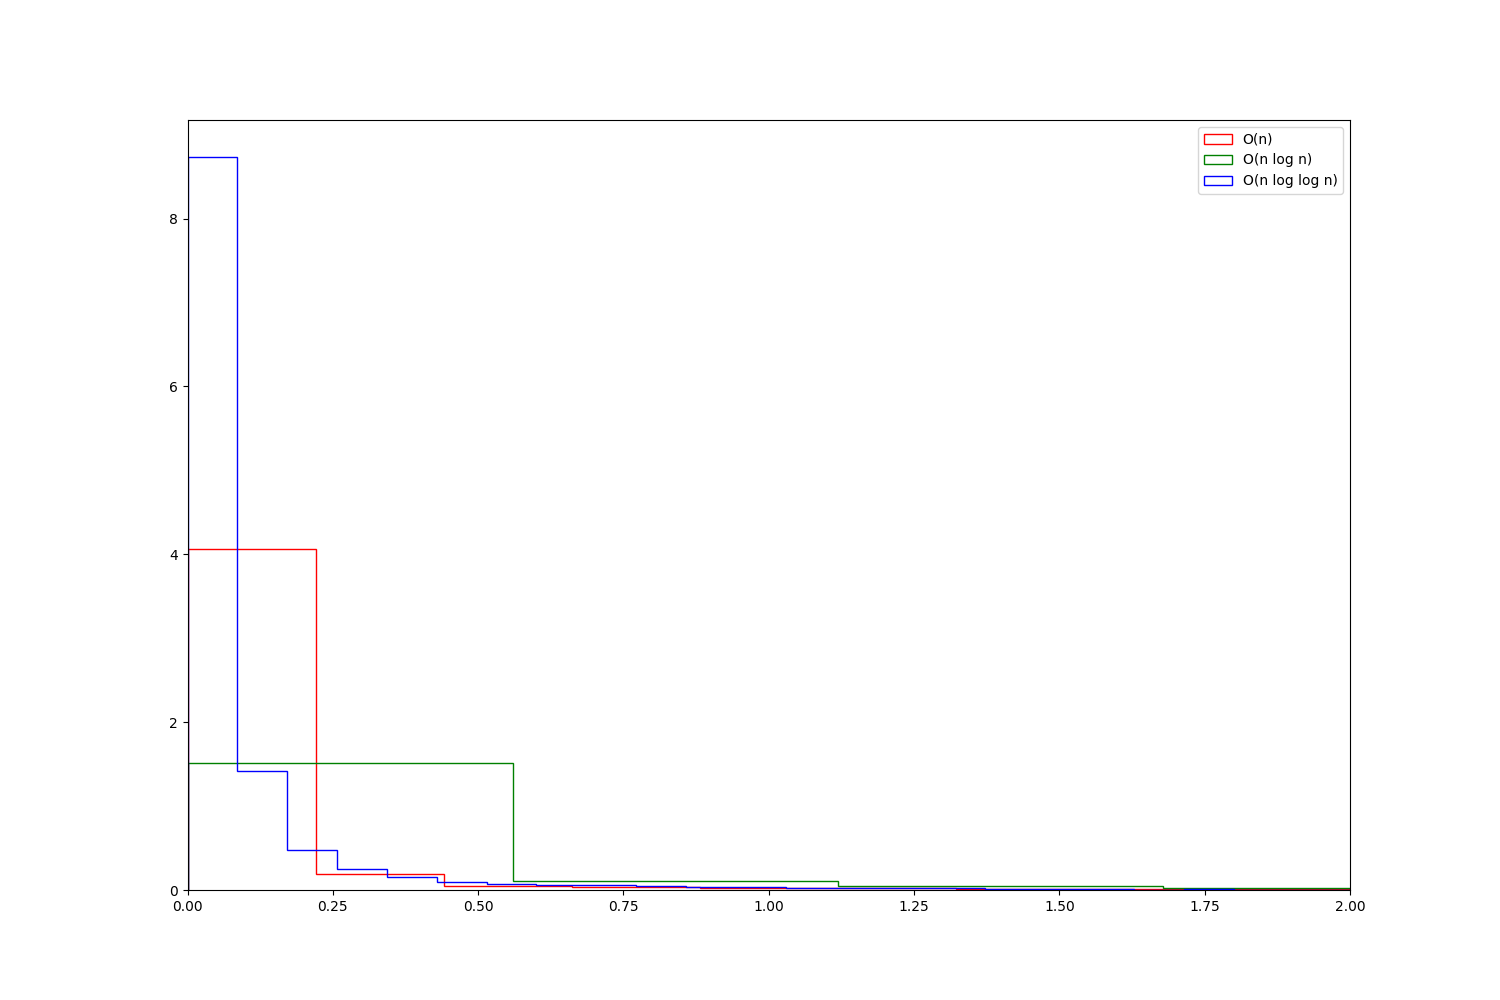
\includegraphics[width=0.44\textwidth]{fig_dist_anal_gauss_statsort.png}
		\end{center}
		\caption{Analysis of algorithm complexity for std sort (left) and stat sort (right) and confirmation that std sort is $O(n \log n)$ and stat sort is $O(n \log \log n)$ for Gaussian distribution.}
		\label{fig6}
		\end{figure}	

                \begin{figure}
		\begin{center}
			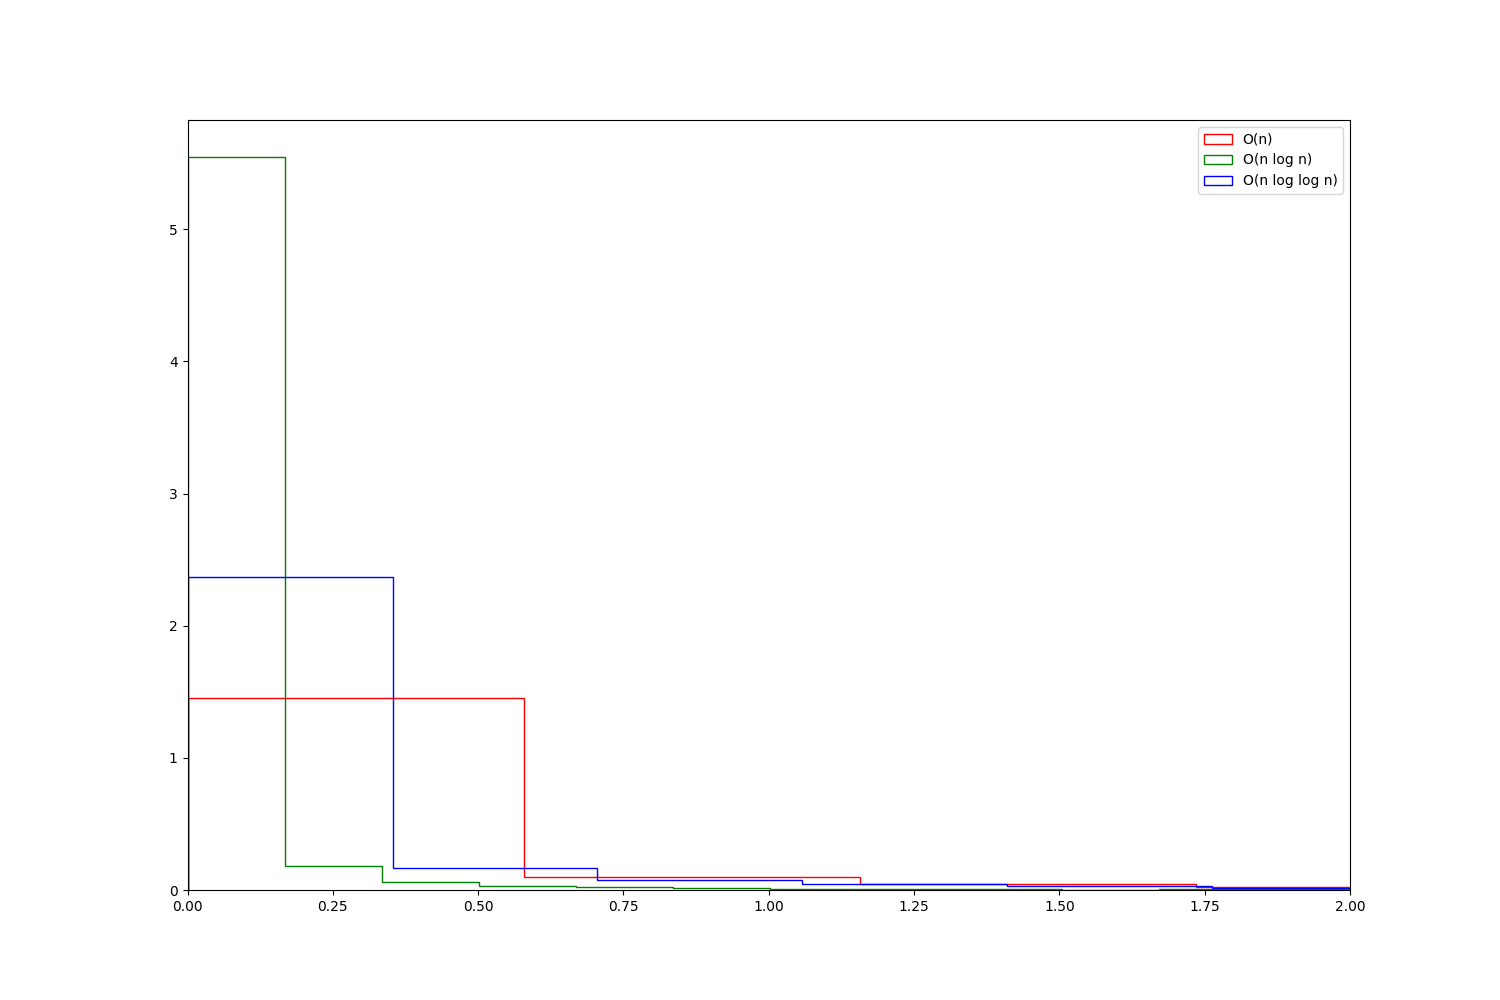
\includegraphics[width=0.44\textwidth]{fig_dist_anal_weird_stdsort.png}
			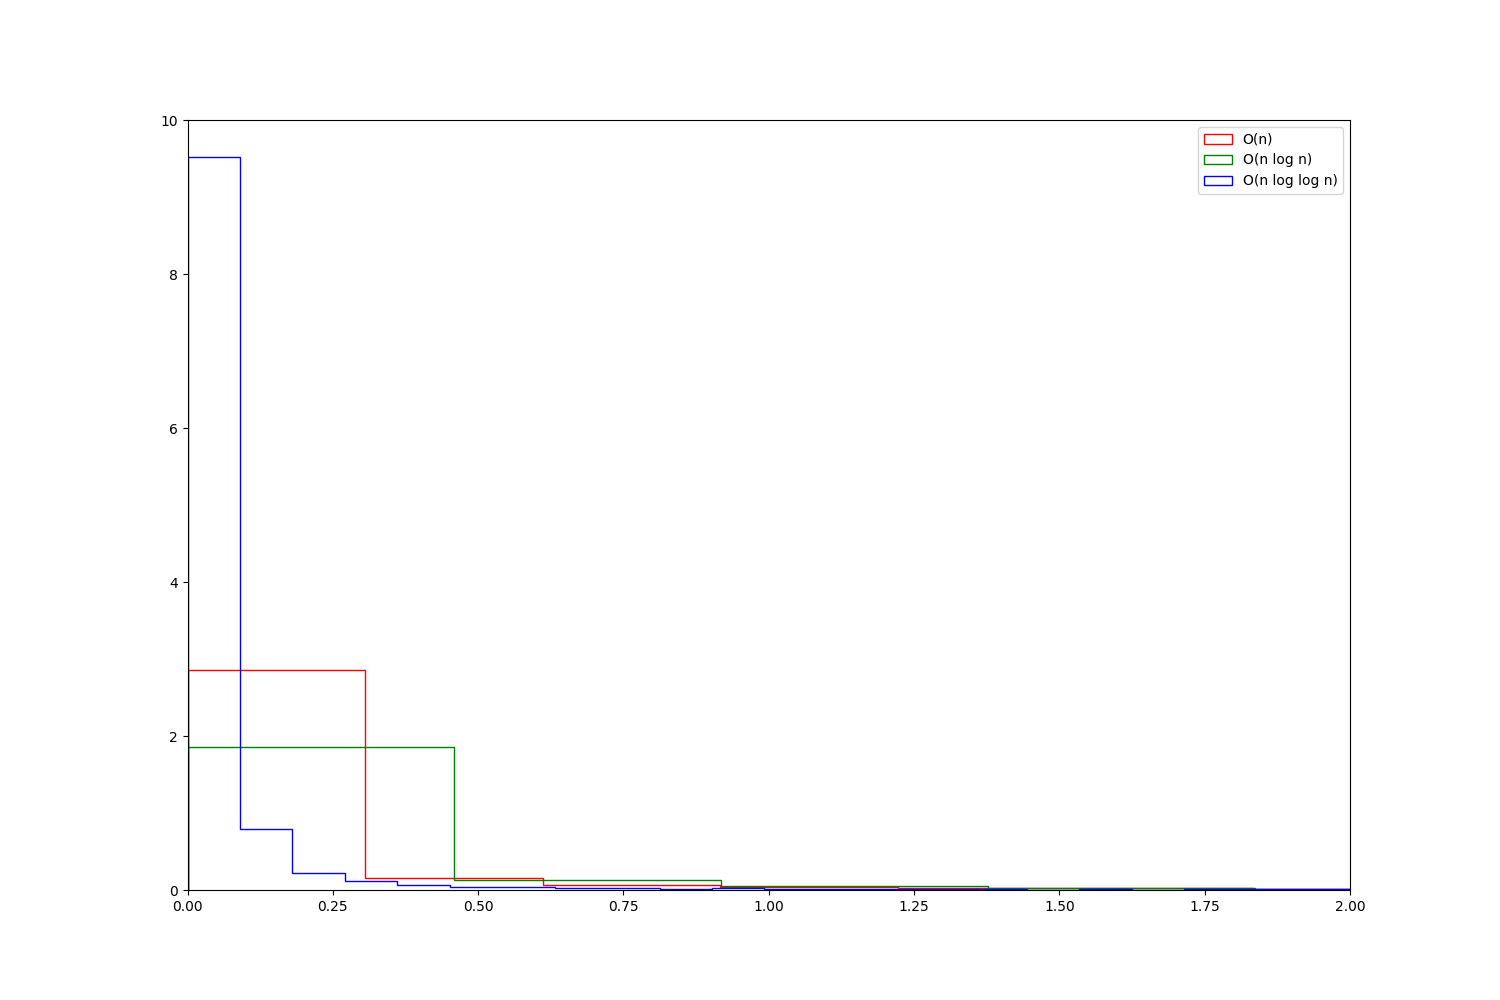
\includegraphics[width=0.44\textwidth]{fig_dist_anal_weird_statsort.png}
		\end{center}
		\caption{Analysis of algorithm complexity for std sort (left) and stat sort (right) and confirmation that std sort is $O(n \log n)$ and stat sort is $O(n \log \log n)$ for additional distribution.}
		\label{fig7}
		\end{figure}	
	\section{Parallelization}
	
	As the initial vector is split into multiple vectors, all the smaller vectors can be sorted in parallel, which makes the statistical sorting algorithm easily parallelizable. As this is quite trivial software engineering work, we will not provide further details in this work, but code for parallelization can be found again on GitHub \cite{peta78b}.

	\section{Discussion \& Future Work}
	
	We introduced statistical sorting and showed from measurements and also by intuition, that its complexity is closer $O(n)$ than $O(n \log n)$ and that it is in fact $O(n \log \log n)$, which is better than any currently known sorting algorithm on average. On average, all known sorting algorithms have a complexity of at least $O(n \log n)$. We also compared it with the C++ implementation of std sort, which has on average $O(n \log n)$ time complexity. We compared statistical and std sort algorithms on three different vector distributions - uniform, Gaussian and an additional one. We also explained why theoretically choosing a variable number of buckets ($\sqrt{n}$) and nesting of the stat algorithm are needed to achieve better performance.
	
	Further work should concentrate on determining the best possible threshold for recursion as well as what algorithm should be used for sorting tiny vectors (if there is a better possibility than C++ std sort). Further work should also look into what happens with vectors of sizes beyond the ones measured in this publication as we showed only intuition beyond the size of vector 500000000.
	
	\section*{Acknowledgement}
	
	The authors would like to thank the Dutch-born people of Amsterdam, Netherlands for the pleasant working environment in the spring of 2023, when the idea for statistical sorting was sparked. The authors would like to thank Grammarly for improving English in this work. The authors would also like to thank Berkeley Public Library, where the publication was partially written, for providing their laptops.
	
\begin{thebibliography}{9}
\bibitem{numrec}
Press, William H. and Teukolsky, Saul A. and Vetterling, William T. and Flannery, Brian P. (2007), Numerical Recipes 3rd Edition: The Art of Scientific Computing, Cambridge University Press, USA

\bibitem{gauss}
Carl F. Gauss (1823), Theoria combinationis observationum: erroribus minimis obnoxiae, Gottingae, H. Dieterich, Print

\bibitem{cppsort}
Geek Writers, std::sort() in C++ STL, \url{https://www.geeksforgeeks.org/sort-c-stl/}

\bibitem{wikisort}
Wikipedia Writers, Sorting algorithm, \url{https://en.wikipedia.org/wiki/Sorting_algorithm}

\bibitem{peta78}
Peter Taraba, Statistical sorting algorithm, \url{https://github.com/peta78/Sorting/tree/main/sorting_publication}

\bibitem{peta78b}
Peter Taraba, Statistical sorting algorithm, \url{https://github.com/peta78/Sorting}

\end{thebibliography}

	
	
\end{document}